\documentclass{article}
\usepackage{ctex}
\usepackage[colorlinks=true, linkcolor=blue, urlcolor=blue]{hyperref}
\usepackage{pgfplots}
\usepackage{graphicx} 
\usepgfplotslibrary{groupplots}
\usepackage{subcaption}
\usepackage{hyperref}
\usepackage{algorithm, algorithmic}
% if you need to pass options to natbib, use, e.g.:
%     \PassOptionsToPackage{numbers, compress}{natbib}
% before loading neurips_2024


% ready for submission
% \usepackage{neurips_2024}


% to compile a preprint version, e.g., for submission to arXiv, add add the
% [preprint] option:
%     \usepackage[preprint]{neurips_2024}


% to compile a camera-ready version, add the [final] option, e.g.:
 \usepackage[final]{neurips_2024}


% to avoid loading the natbib package, add option nonatbib:
%    \usepackage[nonatbib]{neurips_2024}


\usepackage[utf8]{inputenc} % allow utf-8 input
\usepackage[T1]{fontenc}    % use 8-bit T1 fonts
\usepackage{hyperref}       % hyperlinks
\usepackage{url}            % simple URL typesetting
\usepackage{booktabs}       % professional-quality tables
\usepackage{amsfonts}       % blackboard math symbols
\usepackage{nicefrac}       % compact symbols for 1/2, etc.
\usepackage{microtype}      % microtypography
\usepackage{xcolor}         % colors



\title{Final Report: An Investigation of grokking phenomenon}
\vspace{-8.5em}
\author{解晟平\  陈全\  何雨桐}
\vspace{-8.5em}
% The \author macro works with any number of authors. There are two commands
% used to separate the names and addresses of multiple authors: \And and \AND.
%
% Using \And between authors leaves it to LaTeX to determine where to break the
% lines. Using \AND forces a line break at that point. So, if LaTeX puts 3 of 4
% authors names on the first line, and the last on the second line, try using
% \AND instead of \And before the third author name.




\begin{document}


\maketitle
\vspace{-1.5em}
\begin{abstract}
 Grokking has been a widely discussed phenomenon in machine learning research, which reflects that the generalization of model can happen far after memorization or overfitting. In this report, we based on the original paper \href{https://arxiv.org/pdf/2201.02177}{Grokking: Generalization Beyond Overfitting on Small Algorithmic Datasets}  and mainly investigate this phenomenon by learning modular addition task: $(x, y) \rightarrow (x + y)\ mod\ p$ . Since the original paper's code is outdated, we have referenced the following reproduction of grokking: \href{https://github.com/Sea-Snell/grokking}{https://github.com/Sea-Snell/grokking}  as the framework for our code, then we add our own implementation to study the effects of different factors, including model structure, optimizers, number of  elements, and we use wandb to visualize our results. Furthermore, we discuss three different explanations of the grokking phenomenon, validate them with our own experiments and find that a sharpness-aware minimization algorithm called AdaSAM can effectively reduce the grokking delay. All the code and supplementary materials are available at: \href{https://github.com/Tsokarsic/miml-project-3}{https://github.com/Tsokarsic/miml-project-3}.
\end{abstract}

\vspace{-1em}
\section{Problem setting}
\vspace{-1em}

Before we show our results ,we first define the problem formally. Assume $p$ is a prime number, what we should do is to train a modular addition calculator using neural network. For the inputs, as the model shouldn't get access to the integer structure during training, we first transfer both the integers$(0, 1, \ldots, p-1) 
$ and the operands$(+,=)$ to one-hot vectors, where we assign"+" as $p$ and "=" as $p+1$, so the dimension of each vector is $p+2$ .Assume there are $n$ elements to be added, the equation will be "${a_1+a_2+\ldots+a_n=} $", and the output should be a number in $(0, 1, \ldots, p-1) $. Therefore, the model can be regarded as a classifier.  For majority tasks, we selected $p=97$ and $n=2$.

For the model structure, we used a 2-layer multi-head transformer decoder model which consists 4 transformer heads and intermediate-dimension=512. For majority of our experiments, we use AdamW with batch size=512, learning rate=$10^{-3}$, Weight decay=1, $\alpha =0.9, \beta=0.98$ as optimizer, with linear learning rate warm-up in first 10 steps and a maximal optimization budget of $10^6$ steps. Due to limitation of computation resources, we decided the end the training process if the validation accuracy maintained at over 98\%.
% \subsection{Retrieval of style files}


% The style files for NeurIPS and other conference information are available on
% the website at
% \begin{center}
%   \url{http://www.neurips.cc/}
% \end{center}
% The file \verb+neurips_2024.pdf+ contains these instructions and illustrates the
% various formatting requirements your NeurIPS paper must satisfy.


% The only supported style file for NeurIPS 2024 is \verb+neurips_2024.sty+,
% rewritten for \LaTeXe{}.  \textbf{Previous style files for \LaTeX{} 2.09,
%   Microsoft Word, and RTF are no longer supported!}


% The \LaTeX{} style file contains three optional arguments: \verb+final+, which
% creates a camera-ready copy, \verb+preprint+, which creates a preprint for
% submission to, e.g., arXiv, and \verb+nonatbib+, which will not load the
% \verb+natbib+ package for you in case of package clash.


% \paragraph{Preprint option}
% If you wish to post a preprint of your work online, e.g., on arXiv, using the
% NeurIPS style, please use the \verb+preprint+ option. This will create a
% nonanonymized version of your work with the text ``Preprint. Work in progress.''
% in the footer. This version may be distributed as you see fit, as long as you do not say which conference it was submitted to. Please \textbf{do
%   not} use the \verb+final+ option, which should \textbf{only} be used for
% papers accepted to NeurIPS.


% At submission time, please omit the \verb+final+ and \verb+preprint+
% options. This will anonymize your submission and add line numbers to aid
% review. Please do \emph{not} refer to these line numbers in your paper as they
% will be removed during generation of camera-ready copies.


% The file \verb+neurips_2024.tex+ may be used as a ``shell'' for writing your
% paper. All you have to do is replace the author, title, abstract, and text of
% the paper with your own.


% The formatting instructions contained in these style files are summarized in
% Sections \ref{gen_inst}, \ref{headings}, and \ref{others} below.

\vspace{-1em}
\section{Experiments}
\vspace{-1em}
\label{gen_inst}

\subsection{Grokking in transformer}
\vspace{-0.5em}
In this section, we reproduce the results in [1]. To be specific, we show the grokking phenomenon of modular addition using the model of transformer and the optimizer of AdamW.

We first investigate the grokking phenomenon when $\alpha = 0.4$. We make experiments with $p$ ranging in $47, 97, 149, 197$. As is shown in \hyperref[fig1:main]{Figure~\ref{fig1:main}}, the grokking phenomenon is clear, as the validation accuracy reaches 1 long after the training accuracy reaches 1. Beyond the original article, we discovered an interesting “double-grokking” phenomenon: when we choose $\alpha$=0.4 we found that the validation accuracy soon reached around $40\%$, and then stayed at that level for a long time until the model finally grok to near $100\%$ accuracy.




\begin{figure}[htbp]
  \centering
  % 第一列
   \begin{subfigure}[b]{0.22\textwidth}
        \centering
    \includegraphics[width=\textwidth]{picture/47,0.4.png}
    \caption{training and validation accuracy when p=47 $\alpha$=0.4}
    \label{fig1:sub1}
  \end{subfigure}
  \hspace{0.5em} % 列之间的间距
  % 第二列
     \begin{subfigure}[b]{0.22\textwidth}
        \centering
    \includegraphics[width=\textwidth]{picture/97 0.4.png}
    \caption{training and validation accuracy when p=97 $\alpha$=0.4}
    \label{fig1:sub2}
  \end{subfigure}
  \hspace{0.5em} % 列之间的间距
  % 第三列
     \begin{subfigure}[b]{0.22\textwidth}
        \centering
    \includegraphics[width=\textwidth]{picture/149 0.4.png}
    \caption{training and validation accuracy when p=149 $\alpha$=0.4}
    \label{fig1:sub3}
  \end{subfigure}
  \hspace{0.5em} % 列之间的间距
  % 第四列
    \begin{subfigure}[b]{0.22\textwidth}
        \centering
    \includegraphics[width=\textwidth]{picture/197 0.4.png}
    \caption{training and validation accuracy when p=197 $\alpha$=0.4}
    \label{fig1:sub4}
  \end{subfigure}
  
  \renewcommand{\figurename}{Figure}
  \caption{Grokking phenomenon with different $p$.
  In the diagram, we use solid lines to represent training accuracy and dashed lines to represent validation accuracy. Each step consists of 100 iterations. The following experimental results adopt this setting as well.}
  \label{fig1:main}
\end{figure}

\vspace{-0.5em}

Meanwhile, when we compare the results using different $p$, we surprisingly find out that as $p$ increases, the training time decreases, which is against our intuition. We infer this phenomena that as the model's parameters remain unchanged, It becomes more difficult for the model to fit the training data solely through memorization rather than understanding when the size of the training dataset increases, which prompt the model to lean more towards finding a solution with stronger generalization ability at the outset. We also found that as $p$ decreases, the accuracy curve became more fluctuating and sharp.




\begin{figure}[htbp]
  \centering
  % 第一列
   \begin{subfigure}[b]{0.22\textwidth}
        \centering
    \includegraphics[width=\textwidth]{picture/97 0.2.png}
    \caption{training and validation accuracy when p=97 $\alpha$=0.2}
    \label{fig2:sub1}
  \end{subfigure}
  \hspace{0.5em} % 列之间的间距
  % 第二列
     \begin{subfigure}[b]{0.22\textwidth}
        \centering
    \includegraphics[width=\textwidth]{picture/97 0.4.png}
    \caption{training and validation accuracy when p=97 $\alpha$=0.4}
    \label{fig2:sub2}
  \end{subfigure}
  \hspace{0.5em} % 列之间的间距
  % 第三列
     \begin{subfigure}[b]{0.22\textwidth}
        \centering
    \includegraphics[width=\textwidth]{picture/97 0.6.png}
    \caption{training and validation accuracy when p=97 $\alpha$=0.6}
    \label{fig2:sub3}
  \end{subfigure}
  \hspace{0.5em} % 列之间的间距
  % 第四列
    \begin{subfigure}[b]{0.22\textwidth}
        \centering
    \includegraphics[width=\textwidth]{picture/97 0.8.png}
    \caption{training and validation accuracy when p=97 $\alpha$=0.8}
    \label{fig2:sub4}
  \end{subfigure}
  
  \renewcommand{\figurename}{Figure}
  \caption{Grokking phenomenon with different training fraction $\alpha$}
  \label{fig2:main}
\end{figure}

\vspace{-0.5em}

%对齐
Then we change $\alpha$ to examine the impact of grokking phenomenon caused by the change of $\alpha$. We observe that as $\alpha$ increases, the grokking time decreases, which means the validation accuracy reaches 1 earlier. This is consistent with the intuition that the more training data, the easier the training process will be. The result are shown in \hyperref[fig2:main]{Figure~\ref{fig2:main}}.

\vspace{-1em}
\subsection{Grokking in different models}
\vspace{-1em}
In this section we applied other models to investigate whether grokking phenomenon still exists. Specifically, we adopt MLP and LSTM to show the results. Our MLP model consists of 2 layers, $512 \rightarrow 512 \rightarrow 99$. The learning rate here is set as $5e-4$ to get more stable results. We can see from \hyperref[fig3:main]{Figure~\ref{fig3:main}}. that grokking still exists in MLP models. We also found that when the training fraction is low, MLP model generalizes twice faster than transformer if we use training steps as standard, and if we consider the total training time, MLP model outweighs transformer more,showing MLP is probably more suitable on solving easy classification problems.

\begin{figure}[htbp]
  \centering
  % 第一列
   \begin{subfigure}[b]{0.22\textwidth}
        \centering
    \includegraphics[width=\textwidth]{picture/mlp 0.2-3.png}
    \caption{training and validation accuracy when p=97 $\alpha$=0.2}
    \label{fig3:sub1}
  \end{subfigure}
  \hspace{0.5em} % 行之间的水平间距
  % 第二列
     \begin{subfigure}[b]{0.22\textwidth}
        \centering
    \includegraphics[width=\textwidth]{picture/mlp 0.4.png}
    \caption{training and validation accuracy when p=97 $\alpha$=0.4}
    \label{fig3:sub2}
  \end{subfigure}
  \hspace{0.5em} % 行之间的垂直间距
  % 第三列
     \begin{subfigure}[b]{0.22\textwidth}
        \centering
    \includegraphics[width=\textwidth]{picture/mlp 0.6.png}
    \caption{training and validation accuracy when p=97 $\alpha$=0.6}
    \label{fig3:sub3}
  \end{subfigure}
  \hspace{0.5em} % 行之间的水平间距
  % 第四列
    \begin{subfigure}[b]{0.22\textwidth}
        \centering
    \includegraphics[width=\textwidth]{picture/mlp 0.8.png}
    \caption{training and validation accuracy when p=97 $\alpha$=0.8}
    \label{fig3:sub4}
  \end{subfigure}
  
  \renewcommand{\figurename}{Figure}
  \caption{Grokking phenomenon in MLP model.}
  \label{fig3:main}
  \vspace{-1em}
\end{figure}

\vspace{-0.5em}

The LSTM model we adopt is a 1-depth layer with intermediate dimension 512. In our LSTM model, as shown in \hyperref[fig4:main] {Figure~\ref{fig4:main}}, grokking phenomenon also exists. The phenomenon is similar to what is shown in the transformer model. However, we can see that the convergence time in both models is longer than that in the transformer model, which may show the superiority of the transformer structure. What is more, the relationship between $\alpha$ and grokking time still holds, i.e. as $\alpha$ increases, grokking time decreases.


\begin{figure}[htbp]
  \centering
  % 第一列
   \begin{subfigure}[b]{0.22\textwidth}
        \centering
    \includegraphics[width=\textwidth]{picture/lstm 0.2.png}
    \caption{training and validation accuracy when p=97 $\alpha$=0.2}
    \label{fig4:sub1}
  \end{subfigure}
  \hspace{0.5em} % 行之间的水平间距
  % 第二列
     \begin{subfigure}[b]{0.22\textwidth}
        \centering
    \includegraphics[width=\textwidth]{picture/lstm 0.4.png}
    \caption{training and validation accuracy when p=97 $\alpha$=0.4}
    \label{fig4:sub2}
  \end{subfigure}
  \hspace{0.5em} % 行之间的垂直间距
  % 第三列
     \begin{subfigure}[b]{0.22\textwidth}
        \centering
    \includegraphics[width=\textwidth]{picture/lstm 0.6.png}
    \caption{training and validation accuracy when p=97 $\alpha$=0.6}
    \label{fig4:sub3}
  \end{subfigure}
  \hspace{0.5em} % 行之间的水平间距
  % 第四列
    \begin{subfigure}[b]{0.22\textwidth}
        \centering
    \includegraphics[width=\textwidth]{picture/lstm 0.8.png}
    \caption{training and validation accuracy when p=97 $\alpha$=0.8}
    \label{fig4:sub4}
  \end{subfigure}
  
  \renewcommand{\figurename}{Figure}
  \caption{Grokking phenomenon in LSTM model}
  \label{fig4:main}
\end{figure}

\vspace{-2em}
\subsection{Effects of different optimizer and regularization techniques}
\vspace{-1em}
In this section, we will discover how different optimizers and regularization methods affect grokking phenomenon. We measure the ability of grokking by the best validation rate after $10^5$  optimization steps. We selected the following optimizers: For SGD-based optimizers,we selected vanilla SGD, SGD with heavy ball momentum and SGD with Nesterov momentum, and we selected momentum 0.99 and learning rate 0.01 in order to fit the optimizer feature. For Adam,we test across different regularization methods and batch-size. We tested mini-batch Adam with batch size=128, vanilla Adam, AdamW with different weight decay rate(0.1 and 1) and Adam with Dropout 0.1. The results are shown in the following figure.

\begin{figure}[htbp]

    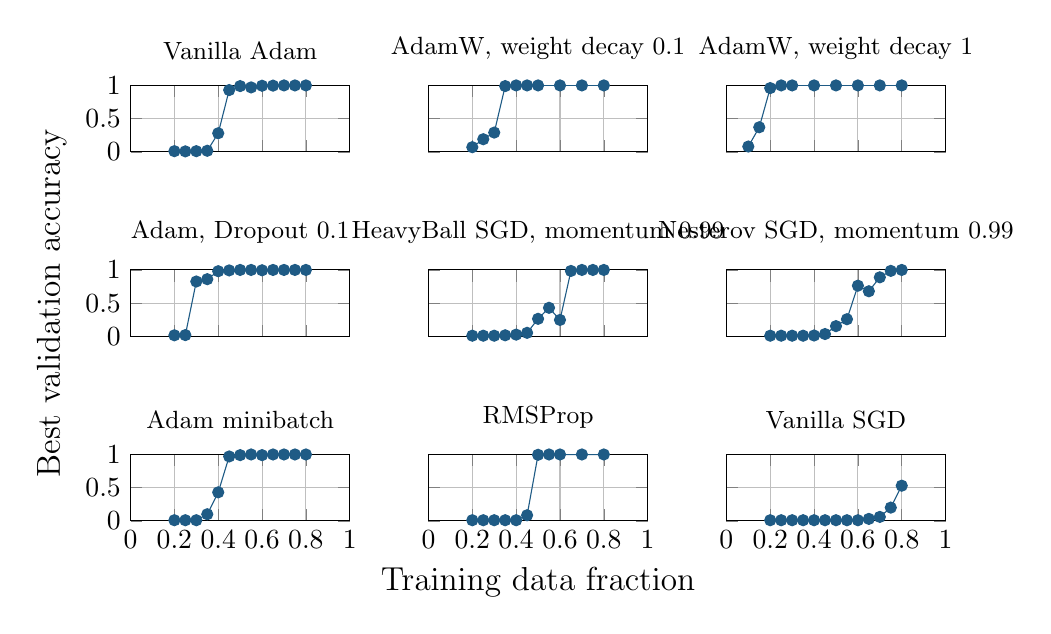
\begin{tikzpicture}
        \begin{groupplot}[
            group style={
                group size=3 by 3, % 3行3列
                horizontal sep=1cm, % 子图之间的水平间距
                vertical sep=1.5cm, % 子图之间的垂直间距
            },
            width=0.36\textwidth, % 设置每个子图的宽度
            height=0.20\textwidth, % 设置每个子图的高度
            xmin=0, xmax=1.0, % 设置 x 轴范围
            ymin=0, ymax=1.0, % 设置 y 轴范围
            xtick={0,0.2,0.4,0.6,0.8,1.0}, % 设置 x 轴刻度位置
            ytick={0,0.5,1.0}, % 设置 y 轴刻度位置
            grid=major,
        ]

            % 第一行第一列,显示坐标轴标签
            \nextgroupplot[
                title={Vanilla Adam},
                 title style={% 设置标题字号为 9 磅
                 font=\fontsize{9pt}{12pt}\selectfont,},
                xticklabels={},
            ]
            \addplot [ color = {rgb:red,42;green,125;blue,183},
            mark=*,] coordinates {(0.2,0.01) (0.25,0.007) (0.3,0.01)(0.35,0.016) (0.4,0.28) (0.45,0.93) (0.5,0.99) (0.55,0.97) (0.6,0.995)(0.65,0.997)(0.7,1)(0.75,1)(0.8,1)};

            % 第一行第二列
            \nextgroupplot[title={AdamW, weight decay 0.1},
                           title style={% 设置标题字号为 9 磅
                              font=\fontsize{9pt}{12pt}\selectfont,},
                           xticklabels={},
                           yticklabels={},]
                \addplot [ color = {rgb:red,42;green,125;blue,183},
            mark=*,]
            coordinates {(0.2,0.07) (0.25,0.19) (0.3,0.29)(0.35,0.99) (0.4,1) (0.45,1) (0.5,1)  (0.6,1)(0.7,1)(0.8,1)};

            %第一行第三列
            \nextgroupplot[title={AdamW, weight decay 1},
                           title style={% 设置标题字号为 9 磅
                              font=\fontsize{9pt}{12pt}\selectfont,},
                           xticklabels={},
                           yticklabels={},]
                \addplot [ color = {rgb:red,42;green,125;blue,183},
            mark=*,] coordinates {(0.1,0.08) (0.15,0.37) (0.2,0.96) (0.25,1) (0.3,1.0)(0.4,1)(0.5,1)(0.6,1)(0.7,1)(0.8,1)};

            %第二行第一列
            \nextgroupplot[title={Adam, Dropout 0.1},
                           title style={% 设置标题字号为 9 磅
                              font=\fontsize{9pt}{12pt}\selectfont,},
                            xticklabels={},
                           ylabel={Best validation accuracy},
                           ylabel style={font=\fontsize{12pt}{12pt}\selectfont,}
                          ]
                \addplot [ color = {rgb:red,42;green,125;blue,183},
            mark=*,] coordinates {(0.2,0.016) (0.25,0.019) (0.3,0.826)(0.35,0.861) (0.4,0.981) (0.45,0.993) (0.5,1) (0.55,1) (0.6,0.995)(0.65,1)(0.7,1)(0.75,1)(0.8,1)};

            %第二行第二列
            \nextgroupplot[title={HeavyBall SGD, momentum 0.99},
                           title style={% 设置标题字号为 9 磅
                              font=\fontsize{9pt}{12pt}\selectfont,}, 
                               xticklabels={},
                           yticklabels={},]
                \addplot [ color = {rgb:red,42;green,125;blue,183},
            mark=*,] coordinates {(0.2,0.01) (0.25,0.01) (0.3,0.01)(0.35,0.016) (0.4,0.026) (0.45,0.053) (0.5,0.264) (0.55,0.430) (0.6,0.247)(0.65,0.985)(0.7,1)(0.75,1)(0.8,1)};

            %第二行第三列
            \nextgroupplot[title={Nesterov SGD, momentum 0.99},
                           title style={% 设置标题字号为 9 磅
                              font=\fontsize{9pt}{12pt}\selectfont,}, 
                            xticklabels={},
                           yticklabels={},]
                \addplot [ color = {rgb:red,42;green,125;blue,183},
            mark=*,] coordinates {(0.2,0.01) (0.25,0.01) (0.3,0.01)(0.35,0.01) (0.4,0.013) (0.45,0.035) (0.5,0.154) (0.55,0.258) (0.6,0.763)(0.65,0.679)(0.7,0.889)(0.75,0.986)(0.8,1)};

             %第三行第一列
             \nextgroupplot[title={Adam minibatch},
                           title style={% 设置标题字号为 9 磅
                              font=\fontsize{9pt}{12pt}\selectfont,},
                           ]
                \addplot [ color = {rgb:red,42;green,125;blue,183},
            mark=*,] coordinates {(0.2,0.01) (0.25,0.01) (0.3,0.01)(0.35,0.10) (0.4,0.43) (0.45,0.97) (0.5,0.99) (0.55,1) (0.6,0.99)(0.65,1)(0.7,1)(0.75,1)(0.8,1)};

            %第三行第二列
             \nextgroupplot[title={RMSProp},
                            title style={% 设置标题字号为 9 磅
                              font=\fontsize{9pt}{10pt}\selectfont,},
                         xlabel={Training data fraction},yticklabels={},xlabel style={font=\fontsize{12pt}{12pt}\selectfont,}
                          ]]
                \addplot [ color = {rgb:red,42;green,125;blue,183},
            mark=*,] coordinates {(0.2,0.01) (0.25,0.01) (0.3,0.01)(0.35,0.01) (0.4,0.01) (0.45,0.085) (0.5,0.995) (0.55,1) (0.6,1)(0.7,1)(0.8,1)};

            %第三行第三列
             \nextgroupplot[title={Vanilla SGD},
                            title style={% 设置标题字号为 9 磅
                              font=\fontsize{9pt}{10pt}\selectfont,},
                         xlabel={},yticklabels={},xlabel style={font=\fontsize{12pt}{12pt}\selectfont,}
                          ]]
                \addplot [ color = {rgb:red,42;green,125;blue,183},
            mark=*,] coordinates {(0.2,0.01) (0.25,0.01) (0.3,0.01)(0.35,0.01) (0.4,0.01) (0.45,0.01) (0.5,0.01) (0.55,0.01) (0.6,0.01)(0.65,0.03)(0.7,0.06)(0.75, 0.20)(0.8,0.53)};
        
        \end{groupplot}
    \end{tikzpicture}
    \vspace{-1em}
\renewcommand{\figurename}{Figure} 
   \caption{best validication rate of different training configurations}    \vspace{-5pt}    

    \label{figure 3}
\end{figure}
\hyperref[figure 3] {Figure~\ref{figure 3}} show results similar to \cite{power2022grokking}[Figure 3, Section 3.3].  Here are our conclusions. Firstly,  AdamW optimizers with an appropriate weight decay outperformed other regularization methods significantly, especially works when the training fraction is small,while other methods such as dropout also increase the capability of generalization. For different optimizers, Vanilla SGD without any momentum struggle to generalize even in large training fraction cases, while momentum based-SGD algorithm and RMSProp can only generalize when the training fraction is relatively large. Finally,we found using small batch-size can slightly enhance generalization when training fraction is small.

\vspace{-1em}
\subsection{Effects of different number of summands}
\vspace{-1em}
In this section, we discovered the effects to grokking with different number of summands, which we take different $n$ defined in problem setting part. In order to reduce the influence of other factors and establish an appropriate unified criterion, we select different $p$ for different $n$, which we choose $p=97$ when $n=2$, $p=23$ when $n=3$, $p=11$ when $n=4,5$, than the dataset size when $p=2,3,4$ are nearly the same, we keep other settings same as the default one in problem settings. To make the influence more clear, we evaluated the effects both on MLP models and transformer models. Our results are shown in \hyperref[fig6:main]{Figure 6}.

\begin{figure}[htbp]
  \centering
  % 第一列
   \begin{subfigure}[b]{0.22\textwidth}
        \centering
    \includegraphics[width=\textwidth]{picture/97 0.4.png}
    \caption{grokking in transformer when p=97 n=2}
    \label{fig6:sub1}
  \end{subfigure}
  \hspace{0.5em} % 行之间的水平间距
  % 第二列
     \begin{subfigure}[b]{0.22\textwidth}
        \centering
    \includegraphics[width=\textwidth]{picture/3 transformer 23.png}
    \caption{grokking in transformer when p=23 n=3}
    \label{fig6:sub2}
  \end{subfigure}
  \hspace{0.5em} % 行之间的垂直间距
  % 第三列
     \begin{subfigure}[b]{0.22\textwidth}
        \centering
    \includegraphics[width=\textwidth]{picture/4 transformer 11.png}
    \caption{grokking in transformer when p=11 n=4}
    \label{fig6:sub3}
  \end{subfigure}
  \hspace{0.5em} % 行之间的水平间距
  % 第四列
    \begin{subfigure}[b]{0.22\textwidth}
        \centering
    \includegraphics[width=\textwidth]{picture/5 transformer 11-2.png}
    \caption{grokking in transformer when p=11 n=5}
    \label{fig6:sub4}
  \end{subfigure}
  
   \begin{subfigure}[b]{0.22\textwidth}
        \centering
    \includegraphics[width=\textwidth]{picture/mlp 0.4.png}
    \caption{grokking in MLP when p=97 n=2}
    \label{fig6:sub5}
  \end{subfigure}
  \hspace{0.5em} % 行之间的水平间距
  % 第二列
     \begin{subfigure}[b]{0.22\textwidth}
        \centering
    \includegraphics[width=\textwidth]{picture/3 mlp 23 m.png}
    \caption{grokking in MLP when p=23 n=3}
    \label{fig6:sub6}
  \end{subfigure}
  \hspace{0.5em} % 行之间的垂直间距
  % 第三列
     \begin{subfigure}[b]{0.22\textwidth}
        \centering
    \includegraphics[width=\textwidth]{picture/4 mlp 11.png}
    \caption{grokking in MLP when p=11 n=4}
    \label{fig6:sub7}
  \end{subfigure}
  \hspace{0.5em} % 行之间的水平间距
  % 第四列
    \begin{subfigure}[b]{0.22\textwidth}
        \centering
    \includegraphics[width=\textwidth]{picture/5 mlp 11.png}
    \caption{grokking in MLP when p=11 n=5}
    \label{fig6:sub8}
  \end{subfigure}
  
  \renewcommand{\figurename}{Figure}
  \caption{Grokking phenomenon with different number of summands}
  \label{fig6:main}
  \vspace{-2em}
\end{figure}



We conclude our observation based on \hyperref[fig6:main]{Figure 6}. First of all, when dealing with larger $n$, the cracking phenomenon in MLP models are still clear, but the gap between generalization and memorization are getting smaller when n grows. While in the transformer model, when $n$ is larger, training and validation accuracy are growing consistently, furthermore, the model fails to perfectly fit $n=5,p=11$ cases as the training accuracy floats around 95\%.  For the total step to generalize, the transformer models always spend more time as n grows, while MLP models spend the most when $n=3$, we infer that this may result from the fact that when n grows, the input data are getting more related to each other, which may improve MLP to predict but may mislead the transformer's self-attention process.


\vspace{-1em}
\section{Explanation to grokking}
\vspace{-0.5em}
\label{headings}
In this section, we discuss three different explanations to the grokking phenomenon. We first discuss the explanation that minima with smaller $\ell_2$ or $\ell_\infty$ norms may generalize better, however,our experiments show that the alignment between parameter norms and generalization ability is not as good as expected,so we further discuss another possible explanation that flatter minima may generalize better and validate by experiments that a sharpness-aware minimization algorithm, AdaSAM, can effectively solve the grokking phenomenon, beating AdamW by a large margin. Finally, we explore an idea that non-linearity may help with the grokking phenomenon, where we observe positive results by replacing ReLU activations by ReLU$^{1.5}$ or ReLU$^2$.

\vspace{-1em}
\subsection{Minima with smaller norm generalize better}
\vspace{-1em}

In machine learning tasks like the modular addition, the model to train is usually over-parameterized, meaning there are many different solutions that minimize training loss. However, not all of the minima can generalize well to out-of-distribution tasks. Consequently, when the training accuracy first becomes 100\%, it is possible that the minimum that the optimization algorithm finds does not generalize well and thus leads to a poor validation accuracy. As the optimization procedure continues, the model parameters can finally tend to minima with certain properties which generalize well, and the validation accuracy finally catches up with the training accuracy.

For example, adding regularization terms, \textit{e.g.}, $\ell_2$ or $\ell_\infty$-norm of the training parameters to the loss function is believed to improve the generalization property. A classical theoretical result states that gradient descent implicitly bias the optimization result to be the minimum with the smallest $\ell_2$-norm when solving linear regression problems. In such cases, the training accuracy may rise quickly due to over-parameterization, and after some delay, the validation accuracy catches up because the parameters finally approach the minimum with the smallest $\ell_2$-norm, thus grokking occurs. Empirically, the experimental results in the previous section have shown that AdamW performs the best to reduce the grokking delay, probably because the weight decay procedure tends to find small $\ell_2$-norm solutions.

\begin{figure}[htbp]
  \centering
    \includegraphics[scale=0.05]{picture/norm and loss.png}
    \renewcommand{\figurename}{Figure}
    \caption{$\ell_2$-norm, $\ell_\infty$-norm and validation loss when p = 97 $\alpha$ = 0.4}
  \label{fig7:main}
\end{figure}


However,Theoretically, the above results may not hold for more complicated models and optimization algorithms, and we also observe in our experiments that though the decrease in validation loss has a similar trend with the parameters $\ell_2$ or $\ell_\infty$ norm, they may not align well enough, as shown in Figure \ref{fig7:main}. 

\textbf{}
\vspace{-1em}
\subsection{Flatter minima generalize better}
\vspace{-1em}
A line of work on generalization property believes flat minima generalize better than sharp ones \cite{keskar2016large}. Sharpness-Aware Minimization (SAM) \cite{foret2020sharpness} finds flatter minima by modifying the objective function, \textit{e.g.}, from $\min_x f(x)$ to $\min_x\max_{\|\epsilon\|_2\le\rho}f(x+\epsilon)$. In order to study the effect of SAM algorithms in accelerating generalization and make fair comparison with AdamW, we choose AdaSAM\cite{sun2024adasam}, a SAM algorithm with adaptive learning rate and momentum acceleration, detailed in Alg.~\ref{alg:AdaSAM}.
\vspace{-0.5em}
\renewcommand{\algorithmicrequire}{\textbf{Input: }}
\renewcommand{\algorithmicensure}{\textbf{Output: }}
\begin{algorithm}

    \caption{AdaSAM}\label{alg:AdaSAM}
    \begin{algorithmic}
    \REQUIRE Initial parameters $x_0$, $m_{-1}=0$, $\hat{v}_{-1}=\epsilon^2$(a small positive scalar to avoid the denominator diminishing), base learning rate $\gamma$, neighborhood size $\rho$ and momentum parameters $\beta_1$, $\beta_2$.
    \ENSURE Optimized parameter $x_{T+1}$.
    \FOR{iteration $t\in\{0,1,2,\cdots,T-1\}$}
    \STATE Sample mini-batch $B=\{\xi_{t_1},\xi_{t_2},\cdots,\xi_{t_{|B|}}\}$;
    \STATE Compute gradient $s_t=\nabla_xf_B(x)\mid_{x_t}=\frac{1}{|B|}\sum_{i\in B}\nabla f_{t_i}(x_t)$;
    \STATE Compute $\delta(x_t)=\rho\frac{s_t}{\|s_t\|}$;
    \STATE Compute SAM gradient $g_t=\nabla_x f_B(x)\mid_{x_t+\delta(x_t)}$;
    \STATE $m_t=\beta_1m_{t-1}+(1-\beta_1)g_t$;
    \STATE $v_t=\beta_2v_{t-1}+(1-\beta_2)g_t^{\odot2}$;
    \STATE $\hat{v}_t=\max(\hat{v}_{t-1},v_t)$;
    \STATE $\eta_t=1/\sqrt{\hat{v}_t}$;
    \STATE $x_{t+1}=x_t-\gamma m_t\odot\eta_t$;
    \ENDFOR
    \end{algorithmic}
    
\end{algorithm}
% \vspace{-0.5em}
\begin{figure}[htbp]
  \centering
  % 第一列
   \begin{subfigure}[b]{0.33\textwidth}
        \centering
    \includegraphics[width=\textwidth]{picture/default-2.png}
    \caption{Acceleration of grokking on pytorch default initialization}
    \label{fig8:sub1}
  \end{subfigure}
  \hspace{1em} % 行之间的水平间距
  % 第二列
     \begin{subfigure}[b]{0.33\textwidth}
        \centering
    \includegraphics[width=\textwidth]{picture/Xavier-3.png}
    \caption{Acceleration of grokking on xavier initialization}
    \label{fig8:sub2}
  \end{subfigure}
  \hspace{1em} % 行之间的垂直间距
  % 第三列
     \begin{subfigure}[b]{0.33\textwidth}
        \centering
    \includegraphics[width=\textwidth]{picture/orthogonal-3.png}
    \caption{Acceleration of grokking on orthogonal initialization}
    \label{fig8:sub3}
  \end{subfigure}
  \hspace{1em} % 行之间的水平间距
  % 第四列
    \begin{subfigure}[b]{0.33\textwidth}
        \centering
    \includegraphics[width=\textwidth]{picture/kaiming-4.png}
    \caption{Acceleration of grokking on kaiming initialization}
    \label{fig8:sub4}
  \end{subfigure}
  
  
  \renewcommand{\figurename}{Figure}
  % \vspace{-0.5em}
  \caption{The effectiveness of AdaSAM optimizer on accelerating generalization and the comparison between different weight initialization methods. }
  \label{fig8:main}
  % \vspace{-2em}
\end{figure}

\vspace{-0.5em}

We compared AdaSAM and AdamW under different initialization settings, whose results is illustrated in Figure \ref{fig8:main}. Though using the same learning rate and momentum parameters, it is observed that under all the experimental settings, AdaSAM generalizes much faster than AdamW.Meanwhile, weight initialization methods also significantly impact the speed of grokking,probably because of the difference on landscape sharpness, and AdaSAM show more improvement in poor initialization cases, which is more robust to landscape sharpness. These results strongly indicate that flatter minima can have better generalization abilities, while minima with small $\ell_2$-norms may not.

\vspace{-1em}
\subsection{Model non-linearity affects generalization}
\vspace{-1em}
As stated in \cite{salah2024controlling}, the nonlinearity of the neural network, which depends on the form of the activation function and the width and depth of the network, can be employed to control the grokking behavior. Consequently, we experimented on a 2-layer MLP network to verify whether the non-linearity in the activation function can help to control the grokking behavior. As illustrated in Figure \ref{fig9:main}, by incorporating non-linearity to the ReLU activation function, the model can really generalize more quickly, where the use of ReLU$(x)^{1.5}$ and ReLU$(x)^2$ perform the best, beating the original ReLU activation by a large margin. 
\begin{figure}[htbp]
  \centering
  % 第一列
   \begin{subfigure}[b]{0.33\textwidth}
        \centering
    \includegraphics[width=\textwidth]{picture/activation accuracy.png}
    \caption{validation acc of different activation functions}
    \label{fig9:sub1}
  \end{subfigure}
  \hspace{1em} % 行之间的水平间距
  % 第二列
     \begin{subfigure}[b]{0.33\textwidth}
        \centering
    \includegraphics[width=\textwidth]{picture/activation loss-2.png}
    \caption{validation loss of different activation functions      }
    \label{fig9:sub2}
  \end{subfigure}
 
  
  \renewcommand{\figurename}{Figure}
  \caption{The effectiveness of activation functions on grokking in a 2-layer MLP network}
  \label{fig9:main}
\end{figure}

\renewcommand{\refname}{Reference}
\bibliographystyle{plain}
\bibliography{reference}

% \section*{References}



% \medskip


% {
% \small


% [1] Power, Alethea et al. “Grokking: Generalization Beyond Overfitting on Small Algorithmic Datasets.” \textit{ArXiv} abs/2201.02177 (2022): n. pag.
% @article{Power2022GrokkingGB,\label{ref1}
 

% [2] Bower, J.M.\ \& Beeman, D.\ (1995) {\it The Book of GENESIS: Exploring
%   Realistic Neural Models with the GEneral NEural SImulation System.}  New York:
% TELOS/Springer--Verlag.


% [3] Hasselmo, M.E., Schnell, E.\ \& Barkai, E.\ (1995) Dynamics of learning and
% recall at excitatory recurrent synapses and cholinergic modulation in rat
% hippocampal region CA3. {\it Journal of Neuroscience} {\bf 15}(7):5249-5262.
% }


%%%%%%%%%%%%%%%%%%%%%%%%%%%%%%%%%%%%%%%%%%%%%%%%%%%%%%%%%%%%


\end{document}


